\subsection{精确外层与有限 inner 的散度进展}

\begin{theorem}[teacher 散度的进展恒等式]
\label{thm:proximal-teacher-progress}
记 $c_\kappa=Z^\kappa$，端点 $\kappa=0,1$ 取 $c_\kappa=1$。对任意候选 $p$，有
\begin{equation}
 \eta\left[D_\kappa(T\Vert q)-D_\kappa(T\Vert p)\right]
 =(1-\eta)D_\kappa(q\Vert p)
 +c_\kappa\left[D_\kappa(m\Vert q)-D_\kappa(m\Vert p)\right].
 \label{eq:proximal-progress-identity}
\end{equation}
若 $D_\kappa(m\Vert p)\le D_\kappa(m\Vert q)$，则 teacher 散度不会增加。精确更新 $p=m$ 且 $q\ne T$ 时严格下降。
\end{theorem}

\begin{proof}
$F(q)=\eta D_\kappa(T\Vert q)$，而 $F(p)=(1-\eta)D_\kappa(q\Vert p)+\eta D_\kappa(T\Vert p)$。由定理~\ref{thm:proximal-barycenter-gap}，$F(q)-F(p)=c_\kappa[D_\kappa(m\Vert q)-D_\kappa(m\Vert p)]$。将 $F(q),F(p)$ 的定义代入并移项，即得恒等式。若目标散度改善，右侧两项非负；若 $p=m$、$q\ne T$，$m\ne q$，则至少第一项严格为正。最后，$m=q$ 会要求 $T_a^\kappa$ 与 $q_a^\kappa$ 成同一比例，概率归一化强制 $T=q$；两个端点同样成立。\hfill$\square$
\end{proof}

这给出了一个纯数学的 finite-inner 条件：降低本轮的 $D_\kappa(m\Vert p)$ 就能提高同一 $D_\kappa$ 下的 teacher 接近度。这里 teacher 散度的方向随 $\kappa$ 改变；一般 $\kappa$ 的保证不能直接替换成每步 $\KL(p\Vert T)$ 都下降。用其他拟合损失获得同一 target，只能在精确求解时自动继承本结论。
\subsection{escort 坐标中的线性轨迹与全局收敛}

对 $\kappa>0$ 定义 escort 分布和幂和
\begin{equation}
 E_\kappa(q)_a=\frac{q_a^\kappa}{S_\kappa(q)},\qquad
 S_\kappa(q)=\sum_aq_a^\kappa.
\end{equation}
$E_\kappa$ 是单纯形上的双射，逆映射为 $q_a\propto E_\kappa(q)_a^{1/\kappa}$。由 $m_a^\kappa=S_a/Z^\kappa$，共同的归一化因子在 escort 中消失，故
\begin{equation}
 E_\kappa(m)=(1-a^{\mathrm{esc}})E_\kappa(q)+a^{\mathrm{esc}}E_\kappa(T),\qquad
 a^{\mathrm{esc}}=\frac{\eta S_\kappa(T)}{(1-\eta)S_\kappa(q)+\eta S_\kappa(T)}.
 \label{eq:proximal-escort-step}
\end{equation}
这是精确式，不是局部近似。$\kappa=1$ 时 $S_1=1$，恢复 $a^{\mathrm{esc}}=\eta$；$0<\kappa<1$ 时，$S_\kappa(q)=\exp((1-\kappa)H_\kappa(q))$，其中 $H_\kappa$ 是 Rényi 熵。因此固定的概率幂插值强度在 escort 坐标中表现为随分布熵改变的有效步幅。

\begin{figure}[htbp]
 \centering
 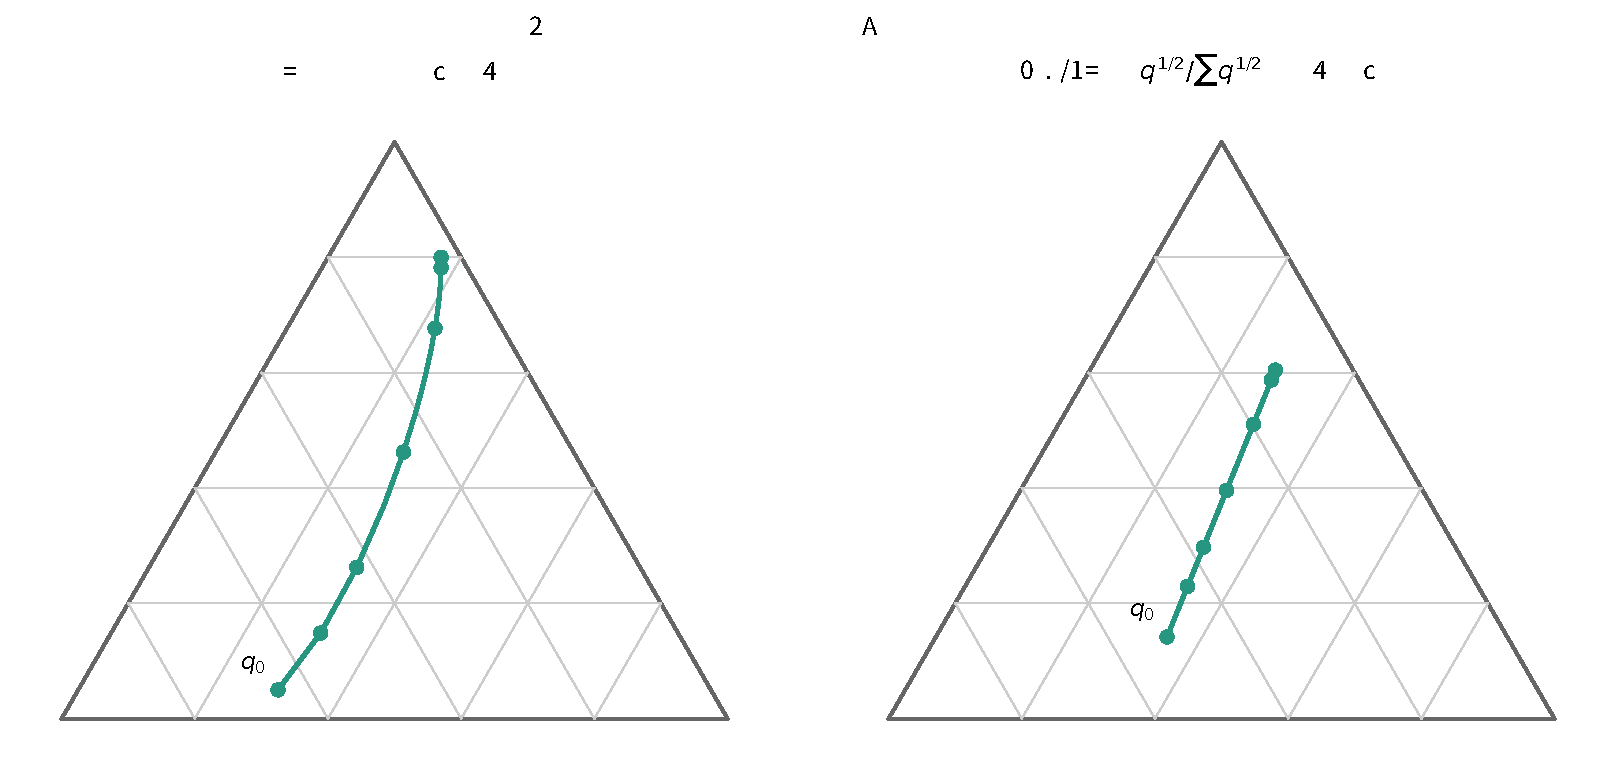
\includegraphics[width=\textwidth]{../../results/proximal-family-geometry/escort.pdf}
 \caption{同一平方根外层轨迹在概率坐标中弯曲，在 escort 坐标中是直线。圆点和数字表示迭代时点。高维分量在固定教师下共享一个进度系数。}
\end{figure}

若 $q_{n+1}=m_{\kappa,\eta}(q_n,T)$，记 $e_n=E_\kappa(q_n)$，则
\begin{equation}
 e_n-e_T=b_n(e_0-e_T),\qquad
 b_n=\prod_{j=0}^{n-1}(1-a_j^{\mathrm{esc}}).
 \label{eq:proximal-escort-orbit}
\end{equation}
这将固定教师下的 $d-1$ 维精确外层轨迹归结为一个标量 $b_n$。对连续自然梯度流，$dq_a/dt=q_a(\rho_a^\kappa-a_\kappa)/\kappa$，所以
\begin{align}
 \frac{d}{dt}q_a^\kappa&=T_a^\kappa-a_\kappa q_a^\kappa,\\
 \frac{d}{dt}S_\kappa(q)&=S_\kappa(T)-a_\kappa S_\kappa(q),\\
 \frac{d}{dt}E_\kappa(q)&=\frac{S_\kappa(T)}{S_\kappa(q)}[E_\kappa(T)-E_\kappa(q)].
\end{align}
改用时间 $\sigma$，$d\sigma/dt=S_\kappa(T)/S_\kappa(q)>0$，就有 $e(\sigma)=e_T+e^{-\sigma}(e_0-e_T)$。离散步式~\eqref{eq:proximal-escort-step} 也位于同一条流轨迹上，对应时间增量 $-\log(1-a^{\mathrm{esc}})$。精确幂均值步因此是这个自然梯度流轨迹的一种时间重参数化，而不只是具有相同起始切线。

\begin{theorem}[teacher 定向的 escort 收缩与误差累积]
\label{thm:proximal-escort-contraction}
令 $d$ 为词表大小，$0<\kappa\le1$，定义度量 $d_\kappa(q,T)=\|E_\kappa(q)-E_\kappa(T)\|_1$。对固定 teacher 的精确更新有
\begin{equation}
 d_\kappa(q_{n+1},T)=(1-a_n^{\mathrm{esc}})d_\kappa(q_n,T)\le c\,d_\kappa(q_n,T),\quad
 c=\frac{(1-\eta)d^{1-\kappa}}{(1-\eta)d^{1-\kappa}+\eta S_\kappa(T)}<1.
\end{equation}
故 $q_n\to T$。若近似更新满足 $d_\kappa(q_{n+1},m(q_n,T))\le\epsilon_n$，则
\begin{equation}
 d_\kappa(q_n,T)\le c^nd_\kappa(q_0,T)+\sum_{j=0}^{n-1}c^{n-1-j}\epsilon_j,
 \qquad
 \limsup_nd_\kappa(q_n,T)\le\frac{\epsilon_\infty}{1-c}
\end{equation}
其中最后一式要求 $\limsup_n\epsilon_n\le\epsilon_\infty$。
\end{theorem}

\begin{proof}
式~\eqref{eq:proximal-escort-step} 给出距离的精确比例。Jensen 不等式给出 $S_\kappa(q)\le d^{1-\kappa}$，因此 $1-a_n^{\mathrm{esc}}\le c$。反复应用得到精确更新的 $c^n$ 界；escort 逆映射连续，故 $q_n\to T$。近似更新时，三角不等式给出 $d_\kappa(q_{n+1},T)\le\epsilon_n+c\,d_\kappa(q_n,T)$，展开得到有限步式。对任意 $\delta>0$，取 $N$ 使 $j\ge N$ 时 $\epsilon_j\le\epsilon_\infty+\delta$。有限个早期项乘以 $c^{n-1-j}$ 后趋于零，后期项的和不超过 $(\epsilon_\infty+\delta)\sum_{i\ge0}c^i$。令 $\delta\to0$ 得极限上界。\hfill$\square$
\end{proof}

这是对固定 teacher 的定向收缩，不声称两个任意 anchor 经同一算子后具有同一个收缩系数；它也不直接等于原概率空间的 TV 收缩。$\kappa\to0$ 时，escort 本身趋于均匀分布，必须重标度才保留信息：
\begin{equation}
 \frac d\kappa\left[E_\kappa(q)_a-\frac1d\right]
 \longrightarrow\log q_a-\frac1d\sum_b\log q_b.
\end{equation}
几何端点就在这些中心化 log 坐标中满足精确比例 $1-\eta$。在任何固定完整支持的 teacher 附近，所有 $\kappa$ 都有 $m(T+\delta,T)=T+(1-\eta)\delta+O(\|\delta\|^2)$，因为 $a_n^{\mathrm{esc}}\to\eta$。它们共享局部收敛率，远处的度量和有效时间则不同。

\begin{figure}[htbp]
 \centering
 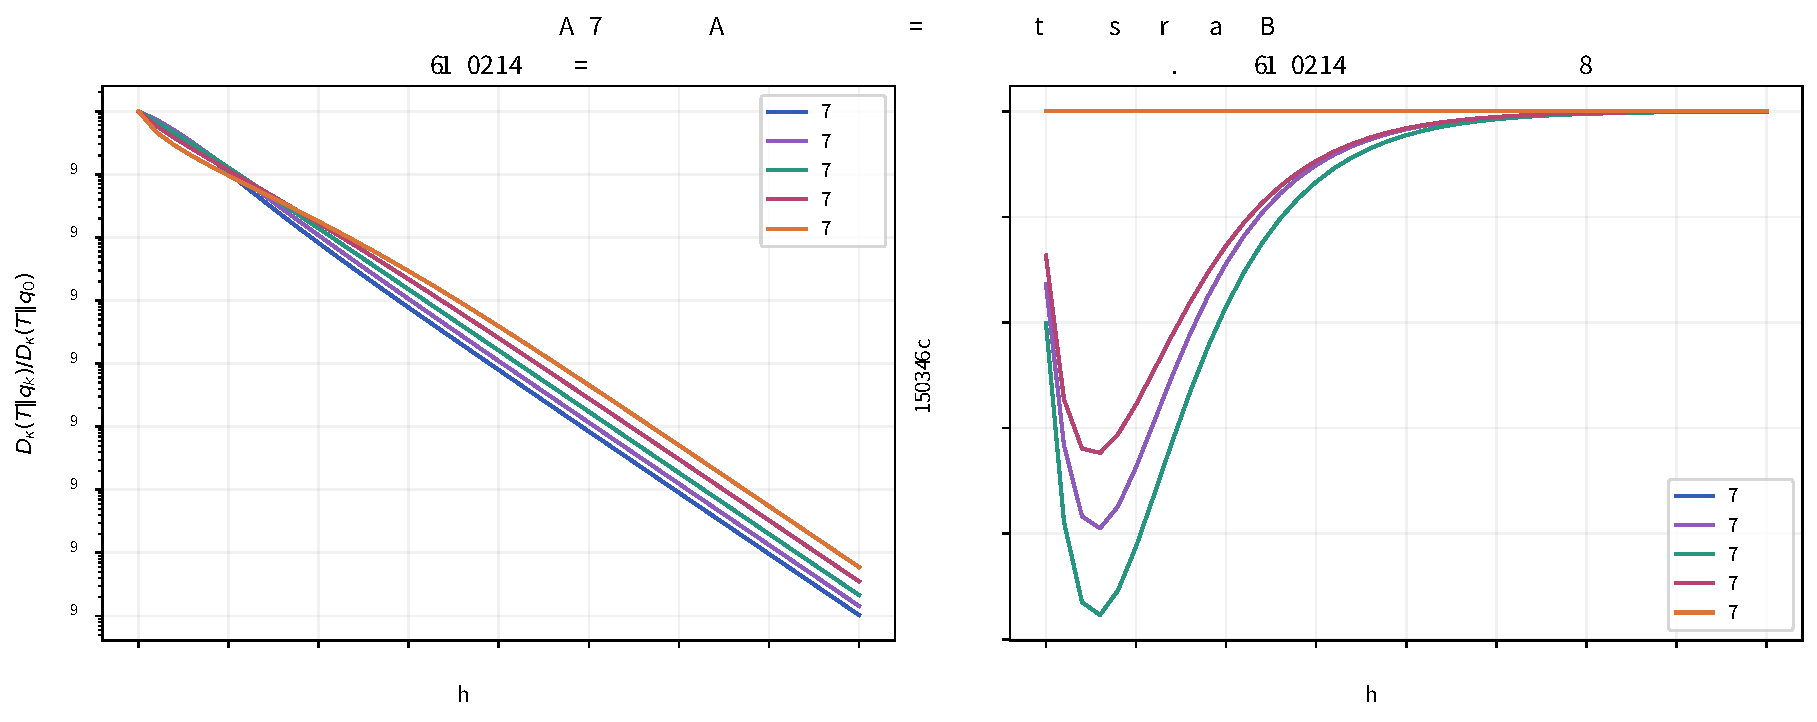
\includegraphics[width=\textwidth]{../../results/proximal-family-geometry/convergence.pdf}
 \caption{精确外层的 teacher 散度单调下降，有效 escort 步幅趋于共同的 $\eta$。每条曲线使用各自的 $D_\kappa$ 并按初值归一化，图中的高低不能直接作为同一任务的训练性能排名。}
\end{figure}
\subsection{共享参数子流形上的自然梯度投影}

独立 token 分布的速度界还可延伸到共享参数的自然梯度流，但需要明确度量。取有限个 prefix、固定权重 $d_s>0$、$\sum_sd_s=1$，将外层分布写成 $q_\theta(a\mid s)>0$。定义
\begin{equation}
 L_\kappa(\theta)=\sum_sd_sD_\kappa(T_s\Vert q_{\theta,s}),\qquad
 \langle v,w\rangle_W=\sum_{s,a}\frac{d_s}{q_{\theta,s,a}}v_{s,a}w_{s,a}.
\end{equation}
记 $J=\partial q_\theta/\partial\theta$，$W=\operatorname{diag}(d_s/q_{\theta,s,a})$，则参数 Fisher 矩阵为 $\mathcal I=J^\top WJ$。令 $v$ 为每个 prefix 上的无约束负自然梯度，$v_{s,a}=q_{\theta,s,a}(\rho_{s,a}^\kappa-\E_{q_{\theta,s}}\rho_s^\kappa)/\kappa$。因为每个 prefix 的 $J$ 列向量分量和为零，$\nabla_\theta L=-J^\top Wv$。

参数自然梯度流采用 Moore--Penrose 广义逆 $\mathcal I^+$ 时，有
\begin{equation}
 \dot\theta=-\mathcal I^+\nabla_\theta L,\qquad
 \dot q_\theta=J\mathcal I^+J^\top Wv=Pv.
\end{equation}
$P$ 是到 $\operatorname{range}(J)$ 的 $W$ 正交投影：令 $B=W^{1/2}J$，则 $W^{1/2}PW^{-1/2}=B(B^\top B)^+B^\top$，后者是普通欧氏正交投影。因此
\begin{equation}
 \|\dot q_\theta\|_W^2\le\|v\|_W^2,\qquad
 \frac{dL}{dt}=-\langle v,Pv\rangle_W=-\|Pv\|_W^2\le0.
\end{equation}
平方根形状满足 $\|v\|_W^2=\sum_sd_s\,4(1-a_s^2)\le4$，所以共享参数的精确自然梯度流也满足 $\|\dot q_\theta\|_W\le2$。更一般地，$0<\kappa\le1/2$ 时平方速度不超过 $1/\kappa^2$。

这个结论控制的是分布流在固定 prefix Fisher 度量下的速度。它不控制参数的欧氏范数，也不自动适用于普通梯度流。共享参数还可能使 $Pv=0$ 而 $q_\theta\ne T$，因此单调性和速度界并不保证无投影误差的 teacher 收敛。离散幂均值 target 的精确 escort 轨迹也不会因这个局部投影结论自动延续到共享参数模型。
